\chapter{Introduction}\label{ch:intro}

\section{Variable stars}
Stars are called variable when there is a detectable change in brightness or color on timescales of the order
of the mean life time of humans~\cite{percy_2007, sterken_1996}.
The first claimed documented variable star is Algol visible with the unaided eye.
There exists ancient Egyptian calendars of lucky and unlucky days that possibly contain the periodicity of Algol\cite{porceddu_2008, porceddu_2018}.
The Cairo Calendar dated to 1244--1163 BC has been shown by Porceddu et al.~\cite{porceddu_2015} to represent Algol as Horus, a sky god and
symbol of kingship,
as seen in the figure~\ref{fig:horus} by matching the actions of Horus and the events witnessed by an observer of Algol.

\begin{figure}[h]
    \centering
    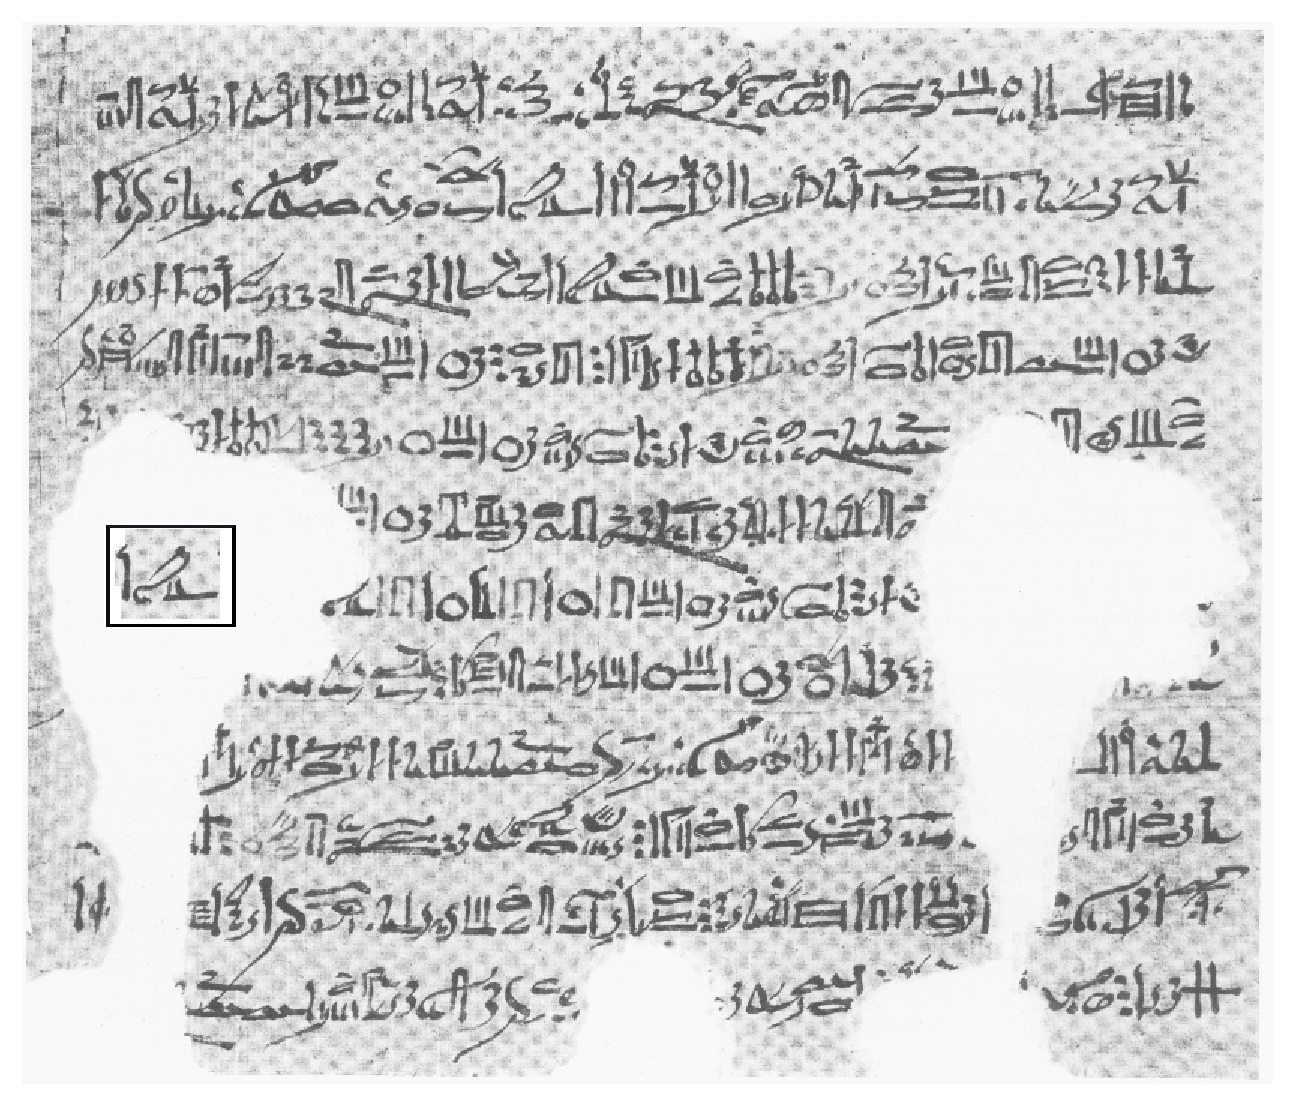
\includegraphics[width=\columnwidth]{figures/horus.eps}
    \caption{Inside the rectangle is the hieratic writing for the word Horus~\protect\cite{porceddu_2015}.}
\label{fig:horus}
\end{figure}

There is some curious relation between ancient Greek stories of the Gorgon Medusa, Perseus, the corresponding constellations, 
and the variable stars Algol and Omicron Ceti or more commonly named Mira (the wonderful).
Wilk~\cite{wilk_1996} suggests that the variability and location in the sky is embedded within the stories themselves.

The first recognized documented variable star, Omicron Ceti,  was recorded in 1596 and again in 1609 by David Fabricius while observing Jupiter.
Fabricius had first recorded Omicron Ceti as a nova, a singular event observed as a bright flash and quick dimming over the next few days,
comparing its significance with a supernova recorded by Tycho Brahe in 1572.
In 1638, Omicron Ceti was rediscovered by Johannes Phocylides Holwarda who found the periodic nature of this star to be approximately 11 months~\cite{hockey_2007}.

%In order to characterize eclipsing binary systems a light curve must be made.
%A light curve is a time series plot of the measured magnitude.

\section{Classifying variability}
Over time there have been several attempts to classify variable stars.
Classification systems reflect the current understanding of the mechanisms behind variability.
The first known formal attempt was made by E.\ C.\ Pickering\cite{sterken_1996, hoffleit_1972} where he classified variable stars into the following categories:
\begin{description}
    \item [Type I] Temporary Stars
\end{description}

\section{Characterizing variability}
Using different algorithms one can distinguish the difference between the types of variable star system.

This demonstrates RR Lyrae
This demonstrates Eclipsing binaries

The relation between orbital mechanics and light curves

This demonstrates solar spots

Complex systems can involve a combination of these different systems.

\section{Eclipsing Binary Characterization}
Binary stars can reveal physical properties by examining the light curves.
Current models use a process called WD code.

In this thesis a modified WD code will be used from the Physics of Eclipsing Binaries (PHOEBE)

\section{O-C calculations}
Observed minus Calculated

\section{Equations of motion}

\section{WD code}
\subsection{Modified WD code}

\section{Pipeline for variable star detection}
\begin{enumerate}
    \item Data needs to be cleaned first.
    \item Align frames
    \item Extract sources
    \item Cross match sources with catalogs
    \item Create Database of known sources
    \item Plot individual light curves
    \item Analyze individual light curves for variability estimation
    \item Sort database given variability ranking
\end{enumerate}




\section{Data Acquisition}
Eclipsing binary optical data acquisition requires an observer to take time series ccd photometry of one target with an observation cadence dependent on the period.

A cadence can be determined by 

For example, the data gathered for this project was collected on multiple nights and observed on the order of hours with evenly timed frames.

\section{Known information of targets examined}

